\chapter{Intégration de l'énergie dans le traitement de requêtes d'un SGBD relationnel}
\label{chap5}

\epigraph{<< Energy and persistence conquer all things. >>}{--- \textup{Benjamin Franklin}}

\NoChapterPrefix \NoChapterNumberInRef {\hypersetup{linkcolor=black} \minitoc}

%% numérotation des figures, des tables et des équations préfixé par le numéro de chapitre
\makeatletter
\renewcommand{\thefigure}{\ifnum \c@section>\z@ \thechapter.\fi
 \@arabic\c@figure}
\@addtoreset{figure}{chapter}
\makeatother

\makeatletter
\renewcommand{\thetable}{\ifnum \c@section>\z@ \thechapter.\fi
 \@arabic\c@table}
\@addtoreset{table}{chapter}
\makeatother

\makeatletter
\renewcommand{\theequation}{\ifnum \c@section>\z@ \thechapter.\fi
 \@arabic\c@equation}
\@addtoreset{equation}{chapter}
\makeatother
%%-----------------------------------------------------------------
%% Résumé
%%-----------------------------------------------------------------

%laisser une page ou deux pages vides, telle est la question !
%\EmptyNewPage
\newpage

%********************************************************************************
%********************************************************************************
\section{Introduction}
Dans les centres de données, la majorité des ressources de calculs et de stockage sont dédiées aux serveurs de bases de données, ce qui rond les SGBDs l'un des principaux consommateurs d'énergie. Cela est dû à la grande quantité de données interrogée par des requêtes complexes; exécutées quotidiennement par un SGBD.
La performance est l'objectif principal qui vient à l'esprit lorsque nous parlons des capacités des SGBDs. Ceci est particulièrement nécessaire pour les scénarios de traitement de requêtes transactionnelles en ligne (\acrshort[hyper=false]{OLTP}) où des centaines et des milliers de transactions comme la mise à jour ou l'insertion de nouveaux tuples dans une relation doivent être exécutées en temps réel. Au fil des années, le temps de traitement des requêtes complexes a diminué grâce à diverses améliorations apportées aux composants matériels et logiciels.

Comme déjà indiqué, les SGBDs existants se concentrent à la haute performance lors de la phase de traitement des requêtes, tout en ignorant généralement la consommation d'énergie. Cependant, des études récentes indiquent qu'une bonne performance n'est plus le seul critère de qualité pour un << bon >> SGBD. Selon le rapport Claremont sur la recherche pour les bases de données, un SGBD éco-énergétique deviendra l'un des principaux domaines de recherche à l'avenir \cite{Claremont08,Abadi16}.

Dans ce chapitre, nous proposons une méthodologie, soutenue par un outil appelé \textit{EnerQuery}, qui crée des bases de données tout en économisant l'énergie lors de la phase de traitement des requêtes. Pour montrer son efficacité, nous mettons en œuvre cette outil dans le module de traitement de requêtes du SGBD libre PostgreSQL. Un modèle mathématique de coût est utilisé pour estimer la consommation d'énergie. Les paramètres de ce dernier sont identifiés par une méthode d'apprentissage automatique. Nous avons mené des expériences intensives en utilisant nos modèles de coûts, et un outil de mesure dédié à calculer l'énergie, tout en basant sur des données de benchmark TPC-H, afin de montrer l’efficacité de nos propositions.

\section{Pourquoi le traitement des requêtes ?}\label{PourquoiOptimisationLogique}
Dans ce chapitre, nous nous concentrons sur le module de traitement de requêtes, qui fait partie des principales composantes d'un SGBD. Plusieurs travaux ont été élaborés dans le domaine de traitement des requêtes depuis le début des années 1970 pour les bases de données traditionnelles. Parmi ces travaux, divers algorithmes et systèmes ont été proposés, tels que le projet \textit{System-R}, dont les résultats ont été largement intégrées dans de nombreux optimiseurs commerciaux (voir \ref{chap2}).

Pour améliorer l'efficacité énergétique lors de l'exécution des requêtes, deux approches sont possibles : (1) nous pouvons soit réduire le temps d'exécution de la requête, (2) soit réduire l'énergie consommée. Le premier aspect a été étudié de manière exhaustive dans plusieurs travaux de littérature, ce qui a conduit au développement des SGBDs relationnels à hautes performances d'aujourd'hui. Le deuxième aspect a été ignoré dans la plupart des études antérieures, mais il est de plus en plus pris en compte dans les projets de recherche récents comme nous avons vu dans le \ref{chap3}.

La phase de traitement de requêtes est une tâche primordiale, car elle est au cœur d'un SGBD. Cette phase doit être exécutée constamment dans le cas des entreprises et des sites web. L'optimiseur de requêtes peut générer un grand nombre de plans d'exécution pour la même requête, ce qui donne de diverses choix de compromis entre les coûts de performance et d'énergie. De plus, un SGBD maintient des statistiques sur les données de la base dans le but d'un traitement efficace des requêtes. Ces informations peuvent être directement utilisées pour dériver le profil d'énergie des requêtes, et aider à la prise de décision liée à la minimisation d'énergie.

\section{Démarche d'intégration de l'énergie dans le traitement de requêtes}\label{Demarche}
Afin de concevoir un traitement de requêtes éco-énergétique, nous proposons tout d'abord un audit de chaque composant, dans le but de vérifier s'il est sensible à l'énergie ou non. Après cette vérification, nous présentons en détail notre méthodologie pour construire le module de traitement de requêtes.

\subsection{Un audit de traitement de requêtes}
Rappelons que le module de traitement de requête est responsable de l'exécution des requêtes suivant un ou plusieurs besoins non fonctionnels, tels que le temps de réponse. Le processus d'exécution d'une requête donnée passe généralement par quatre étapes principales: (i) l'analyse syntaxique, (ii) la réécriture, (iii) la planification et l'optimisation et (iv) l'exécution (cf. \ref{fig:postgres-query-optimizer}). Pour illustrer ces étapes, nous considérons comme une étude de cas le SGBD PostgreSQL\footnote{\url{https://www.postgresql.org/}}.

\begin{figure}
	\centering
	\includegraphics[scale=0.55]{chapitre5/chap5Fig/postgres-query-optimizer.pdf}
	\caption{Étapes de traitement de requêtes dans PostgreSQL.}
	\label{fig:postgres-query-optimizer}
\end{figure}

PostgreSQL est un système de gestion de base de données relationnelle et objet. C'est un outil libre et open-source développé à l'université de Californie à Berkeley par une équipe sous la direction de Michael Stonebraker en 1985. Le nom original était POSTGRES et fut renommé Postgres95. Ce dernier fut changé à la fin de 1996 en PostgreSQL. Il supporte diverses plates-formes matérielles et différents systèmes d'exploitation. PostgreSQL est entièrement conforme à ACID (atomicité, cohérence, isolation et durabilité), avec la prise en charge de nombreuses fonctionnalités comme les clés étrangères, jointures, vues matérialisées, triggers, récupération ponctuelle, tablespaces, réplication asynchrone, transactions imbriquées, sauvegardes en ligne, etc\footnote{\url{https://www.postgresql.org/docs/current/static/intro-whatis.html}}.

% add examples from PostgreSQL source code at each step
% Postgres:
% 2 Query planning in postgreSQL: Optimizing query execution to improve the energy efficiency of database management systems - Master
% Puissance-performance tradeoff in database systems - Master
% A3.pdf
\subsubsection{Analyse syntaxique}\label{subsec:Parse}
L'analyseur syntaxique doit vérifier la chaîne de caractères de la requête pour valider sa syntaxe à l'aide d'un ensemble de règles de grammaire.  Si la syntaxe est correcte, un \textit{arbre syntaxique} est construit et retourné. La fonction responsable de cette tâche dans PostgreSQL est : \texttt{raw\_parser()} située dans le fichier : \path{src/backend/parser/parser.c}. L'analyseur défini dans \texttt{gram.y} et \texttt{scan.l} est construit en utilisant les outils Unix \texttt{bison} et \texttt{flex}. Après la fin de la tâche d'analyseur, le processus de transformation prend l'arbre syntaxique en entrée et fait l'interprétation sémantique nécessaire pour comprendre quelles tables, fonctions et opérateurs référencés par la requête. La structure de données construite pour représenter cette information est appelée \textit{arbre de requête}. La fonction de transformation nommée \texttt{parse\_analyze()} est située dans le fichier \path{src/backend/parser/analyze.c}.  Le coût de cette phase est généralement ignoré par le SGBD car elle se termine très rapidement. Nous suivons la même logique et nous supposons que la consommation d'énergie de cette étape est négligeable.

\subsubsection{Réécriture}\label{subsec:Rewrite}
La phase de réécriture (ou simplification) des requêtes traite l'arbre remis par l'étape d'analyse syntaxique et le réécrit à un autre arbre en utilisant un ensemble de règles. Ces dernières sont définies par l'utilisateur ou le système. Cette phase basée sur des règles est également utilisée dans la réécriture des requêtes dans le cas des vues matérialisées. La fonction de réécriture est nommée \texttt{QueryRewrite()} définie dans le fichier \path{src/backend/rewrite/rewriteHandler.c}. Quant à l'étape précédente, le coût est ignoré en raison de l'achèvement rapide de cette phase.

\subsubsection{Planification/optimisation}\label{subsec:PlanOptimize}
La tâche du planificateur/optimiseur est de créer un plan d'exécution optimal. Une requête SQL donnée peut effectivement être exécutée de différentes manières, dont chacune va produire le même ensemble de résultats. La tâche de l'optimiseur est d'estimer le coût de l'exécution de chaque plan en utilisant une approche basée sur les coûts, et de trouver celle qui doit être exécutée rapidement.

\paragraph{Planification}
Le planificateur commence par générer des plans d'exécution pour la lecture de chaque relation individuelle (table) utilisée dans la requête. Les plans possibles sont déterminés par les \textit{indexes} disponibles sur chaque relation. Il y a toujours la possibilité d'effectuer un \textit{accès séquentiel} sur une relation, donc un plan de accès séquentiel est toujours créé. Si la requête nécessite la jointure de deux ou plusieurs relations, tous les plans possibles pour joindre ces relations sont générés. Les stratégies de jointure disponibles dans PostgreSQL sont: \textit {jointure par boucle imbriquée}, \textit{jointure par fusion} et \textit{jointure par hachage}. Lorsque la requête implique plus de deux relations, le résultat final doit être construit par un arbre de jointures, chacune avec deux entrées. Le planificateur examine les différentes séquences de jointure possibles pour trouver le moins cher en terme de coût. Si la requête utilise un nombre de relations moins d'un certain seuil défini (fixé à 12 relations dans PostgreSQL), une recherche quasi-exhaustive est effectuée pour trouver les meilleures séquences de jointure; autrement, un algorithme heuristique à base de génétique est utilisé.

Pour étudier les effets de ces stratégies de recherche, considérons la requête \textit{Q8} du benchmark TPC-H \cite{TPCH}. C'est une requête complexe qui implique la jointure de 7 tables. Nous modifions le planificateur de PostgreSQL selon trois manières : (i) la recherche d'un plan d'exécution en utilisant la stratégie du SGBD actuelle (ii) en utilisant l'algorithme génétique, et (iii) manuellement en forçant le planificateur de choisir un certain plan. Pour chaque stratégie, nous calculons son temps d'exécution et sa consommation totale d'énergie lors de l'exécution de la requête sur une base de données d'une taille de 10 Go. Les résultats sont présentés dans le \ref{tab:plan-algo}.

\begin{table}
\centering
\caption {Planification de la requête \textit{Q8} de TPC-H avec différentes stratégies de recherche.} \label{tab:plan-algo}
\begin{tabular}{lll}
    \toprule
    \textbf{Stratégie de recherche} & \textbf{Temps de planification (s)} & \textbf{Énergie (J)} \\
    \midrule
    Par défaut & 0,110006 & 5200,362\\ 
	Algorithme génétique & 0,977013 & 5387,648 \\ 
    Manuelle & 0,092054 & 5160,036 \\
    \bottomrule
\end{tabular}
\end{table}

D'après le tableau, on peut constater que la stratégie de choix d'un plan de requête manuel donne les meilleurs résultats, en terme de temps et d'énergie. Alors que la stratégie de recherche par défaut (semi-exhaustive) conduit à un temps d'exécution et de consommation d'énergie un peu plus élevée. L'algorithme génétique donne les pires résultats dans cet exemple, peut-être en raison du petit nombre de tables présent dans la requête, puisque cette stratégie est utilisée par le SGBD où il y a plus de 12 tables. Compte tenu de ce petit nombre de tables, si nous allons dans les bases de données opérationnelles réelles où il y a une centaine de tables, la stratégie de recherche utilisé par le planificateur peut conduire à une consommation d'énergie notable. Ainsi, la stratégie de recherche des plans d'exécution de requêtes manuellement par l'administrateur de base de données est recommandée dans les grandes bases de données pour gagner en efficacité énergétique.

\paragraph{Optimisation}
Pour évaluer le temps de réponse pour chaque plan d'exécution, des fonctions de coût sont définis pour chaque opérateur SQL basique. La formule générale pour estimer le coût de l'opérateur $op$ peut être exprimée comme:
\begin{equation}
 Co\hat{u}t_{op} = \alpha \times E/S \: \oplus \: \beta \times CPU \: \oplus \: \gamma \times Com
\end{equation} 
Où $E/S$, $CPU$ et $Com$ sont des estimations pour le nombres de pages, nombres de tuples et de messages de communication, respectivement, nécessaires pour exécuter l'opérateur $op$. Ils sont généralement calculés à l'aide des statistiques de base de données et des formules de sélectivité. Les coefficients $\alpha$, $\beta$ et $\gamma$ sont utilisés pour convertir les estimations à l'unité souhaitée (par exemple, le temps, l'énergie, etc). $\oplus$ représente la relation entre les paramètres (linéaires, non-linéaires).

L'optimiseur de PostgreSQL utilise cinq types de paramètres dans son modèle de coût, $T \in \{s, r, t, i, o\}$. Le coût d'un opérateur $op$ dans le plan de requête est calculé comme suit :
\begin{equation}
 Co\hat{u}t_{op} = \sum_{i=1}^{T} c_{i} \times n_{i}
\end{equation} 
Où $n$ représente l'estimation de coût d'opérations de type $T$ requises pour exécuter l'opérateur, et $c$ est le coefficient de coût de performance pour le même type. Les fonctions de calcul des coûts d'un opérateur seront représentées dans la \ref{sec:cost-model-param}. Le \ref{tab:postgres-cost-param} donne un aperçu des types d'opérateur définis dans PostgreSQL et les valeurs par défaut des coefficients de coût de performance. Le coût total estimé d'une requête est donc la somme des coûts des opérateurs individuels dans le plan d'exécution.

\begin{table}
\centering
\caption {Présentation des paramètres de modèle de coût de PostgreSQL.} \label{tab:postgres-cost-param}
\begin{tabular}{llll}
    \toprule
    \textbf{\textit{T}} & \textbf{Désignation} & \textbf{Définition} & \textbf{\textit{c}} \\
    \midrule
    $s$ & seq\_page\_cost        & le coût d'E/S pour accéder séquentiellement à une page  & 1,0 \\
    $r$ & random\_page\_cost     & le coût d'E/S pour accéder aléatoirement à une page     & 4,0 \\
    $t$ & cpu\_tuple\_cost       & le coût CPU pour traiter un tuple                       & 0,01 \\
    $i$ & cpu\_index\_tuple\_cost & le coût CPU pour traiter un tuple via un accès index    & 0,005 \\
    $o$ & cpu\_operator\_cost    & le coût CPU pour effectuer une opération (ex : hachage) & 0,0025 \\
    \bottomrule
\end{tabular}
\end{table}

Les paramètres des coefficients et leur relation peuvent être obtenus en utilisant diverses techniques telles que la calibration, la régression et les statistiques. Ainsi, un modèle de coût d'énergie doit être défini à ce niveau, avec les nouveaux paramètres $T$ les plus pertinents.

L'arbre du plan d'exécution final est constitué des opérations d'accès séquentiels ou d'accès par index des relations de base, plus des opérations de jointure par boucle imbriquée, fusion ou hachage, ainsi que des étapes auxiliaires, tels que les opérations de tri ou d'agrégation.

\subsubsection{Exécution}\label{subsec:Executor}
L'exécuteur prend le plan créé par le planificateur/optimiseur et le traite récursivement pour extraire l'ensemble de tuples requis dans un mécanisme de \textit{pipeline}. Chaque fois qu'un nœud du plan est appelé, il doit livrer le prochain tuple, ou signaler qu'il n'y a plus de tuples à livrer. Les requêtes complexes peuvent impliquer de nombreux niveaux de nœuds dans leurs plan d'exécution, mais l'approche générale reste la même : chaque nœud calcule et retourne sa prochaine sortie de tuple, à chaque fois qu'il est appelé. Chaque nœud est également responsable de l'application des expressions de sélection ou de projection qui ont été attribuées par le planificateur.

Pour étudier l'effet de l'étape d'exécution sur l'éco-conception d'un optimiseur de requêtes, nous considérons un exemple de requête \textit{Q22} issue du benchmark TPC-H.
La \ref{fig:q22-plan-pl} présente le plan d'exécution renvoyé par l'optimiseur de requête de PostgreSQL. Comme nous l'avons montré dans le \ref{chap4}, la consommation d'énergie est directement influencée par le modèle d'exécution du SGBD. Par conséquent, le plan d'exécution peut être divisé en un ensemble de segments, nous nous référons à ces segments comme \textit{pipelines}. Ces dernières correspondant à l'exécution simultanée d'une séquence contiguë d'opérateurs.
La segmentation du pipeline du plan d'optimiseur pour la requête \textit{Q22} est représentée sur la \ref{fig:q22-plan-pl}. Dans cette dernière, il y a 4 pipelines, et l'ordre d'exécution de ces pipelines est géré par les opérateurs de blocage (par exemple, PL3 ne peut débuter jusqu'à ce que PL2 se termine).

Dans notre étude précédente (cf. \ref{chap4}), nous avons montré que \textit{lorsqu'une requête passe d'un pipeline à l'autre, sa consommation d'énergie change aussi}. Lors de l'exécution d'un pipeline, la consommation d'énergie a généralement tendance à être constante. Par conséquent, ce modèle d'exécution de pipeline est très important, car il a un impact direct sur la consommation d'énergie lors de l'exécution d'une requête. L'éco-conception d'un optimiseur de requête devrait prendre en considération la stratégie d'exécution. Cet aspect n'est pas pris en charge dans les travaux de Xu \textit{et al.} \cite{Xu10b}.

\begin{figure}
	\centering
	\includegraphics[scale=0.6]{chapitre5/chap5Fig/q22-plan-pl.pdf}
	\caption{Plan d'exécution du requête \textit{Q22} issue du benchmark TPC-H avec l'annotation de pipeline correspondante.}
	\label{fig:q22-plan-pl}
\end{figure}

\section{Méthodologie de conception d'un module de traitement de requêtes éco-énergétique}\label{sec:Methodology}

Dans cette section, nous décrivons la méthodologie de conception et la mise en œuvre de notre proposition dans le SGBD PostgreSQL. Comme nous l'avons mentionné ci-dessus, les phases de planification/optimisation et d'exécution ont un impact sur la consommation d'énergie, et doivent être prises en compte dans la conception d'un module de traitement de requêtes éco-énergétique. Le workflow de notre méthodologie est décrit dans la \ref{fig:methodo-postgres}. Nous avons étendu le module de traitement de requêtes de PostgreSQL pour inclure un modèle de coût estimant l'énergie des opérateurs SQL. Nous avons aussi modifié le processus de sélection des plans d’exécution \textit{mono-objectif} en un processus \textit{multi-objectifs} tout en incluant la dimension énergétique. Notre démarche ne génère pas de frais généraux au processus de traitement de requêtes car nous avons implémenté notre modèle énergétique à côté du modèle de performance existant, pour ne pas refaire les calculs pour chaque opérateur.

\begin{figure}
	\centering
	\includegraphics[scale=0.55]{chapitre5/chap5Fig/dbms-flow.pdf}
	\caption{La méthodologie de conception}
	\label{fig:methodo-postgres}
\end{figure}

\subsection{Modèle de coût d'énergie}
Dans cette section, nous présentons notre méthodologie pour l'estimation de la consommation d'énergie des requêtes dans PostgreSQL. Nous nous sommes basé sur notre démarche introduite dans le \ref{chap4} pour construire notre modèle. Les caractéristiques de ce modèle comprennent: (i) la segmentation d'un plan d'exécution en un ensemble de pipelines, (ii) l'utilisation des paramètres de pipeline pour construire le modèle en utilisant des techniques d'apprentissage automatique (\textit{hors ligne}), et (iii) l'estimation de l'énergie du nouveau pipeline en se basant sur le modèle de coût final (\textit{en ligne}). Les fonctions de régression et de calibration sont les mêmes que celles utilisées dans le \ref{chap4}.

%\subsubsection{Segmentation des pipelines}
\subsubsection{Paramètres du modèle de coût}\label{sec:cost-model-param}
Étant donné une requête SQL, l'optimiseur de requête est responsable de l'estimation des coûts d'E/S et de CPU pour chaque opérateur algébrique de base. Notre stratégie pour la modélisation d'énergie est d'étendre le modèle de coût de ces opérateurs qui sont intégrés dans le SGBD PostgreSQL, afin d'estimer sa consommation d'énergie.
Pour chaque opérateur, les paramètres dans l'\ref{eq:cost-model} (les coûts d'E/S et de CPU) doivent être modifiés en fonction de son implémentation et comportement d'exécution. La suite de cette section sera consacrée à présenter des modèles d'énergie pour un ensemble d'opérateurs relationnels de base.

\paragraph{Accès séquentiel} L'opération d'accès séquentiel parcourt la relation complète telle qu’elle est stockée sur disque, puisque chaque page et tuple doivent être examinés. Le coût d'E/S est égal au nombre de pages dans la relation ($p$), et le coût CPU est égal au nombre de tuples ($t$).
\paragraph{Accès par index} L'opération d'accès par index réalise un parcours d'un arbre d'index, passe à travers des nœuds feuilles pour trouver toutes les entrées correspondantes, et récupère les données correspondantes de la table. Pour chaque index, le nombre de tuples est déterminé par la fraction de tuples dans une relation qui satisfait les clauses de restriction. Cette quantité fractionnaire est appelée << sélectivité >> ($f$).
\paragraph{Accès par bitmap} Un accès par bitmap récupère tous les pointeurs de ligne dans l’index en une seule fois, les trie en mémoire en utilisant une structure bitmap, puis visite les lignes dans la table en suivant l’ordre de leur emplacement physique. Puisque l'accès par bitmap est basé sur l'accès par index, ses coûts d'E/S et de CPU sont calculés de la même façon.
\paragraph{Jointure par boucle imbriquée} La jointure par boucle imbriquée joint deux tables en récupérant le résultat d’une table ($inner$), et en recherchant chaque ligne de la première table dans la seconde ($outer$). Pour toutes les stratégies de jointure, l'estimation de la taille des deux relations $inner$ et $outer$ est obtenue par la multiplication de la taille originale de la relation par la sélectivité $f$ de chaque clause de restriction dans la jointure. Le coût d'E/S dans ce type de jointure est la somme du coût de la relation $inner$ et $outer$, le coût CPU est la multiplication de nombres de tuples dans chaque relation.
\paragraph{Jointure par tri-fusion} La jointure par tri-fusion combine deux listes triées comme une fermeture éclair. Les deux côtés de la jointure doivent être triés par les prédicats de jointure. Le coût d'E/S est la somme des coûts de la relation $inner$ et $outer$. Le coût CPU est égal à la somme des coûts pour trier les tuples des deux relations.
\paragraph{Jointure par hachage} La jointure de hachage charge les tuples candidats d’un côté de la jointure dans une table de hachage dont chaque enregistrement est ensuite testé avec l’autre côté de la jointure. Le coût d'E/S est le coût de lecture des deux relations $outer$ et $inner$, et le coût CPU est égal à la somme des coûts dans la phase de construction de la table de hachage $n_hash$ plus la phase de sondage des tuples satisfaisants les clauses de jointures $p_hash$.
\paragraph{Tri} Cet opérateur trie l’ensemble de données ($s$) sur les colonnes mentionnées dans la requête. L'opération a besoin d’une quantité de mémoire tampon $m$ pour matérialiser le résultat intermédiaire. Deux cas sont distingués, si l'opération de tri peut se faire dans la mémoire ($s < m$) alors PostgreSQL applique l'algorithme de tri rapide, où le coût d'E/S est nul. Sinon, le coût de sauvegarde et de la relecture de données s'ajoutent au coût d'E/S. Dans les deux cas, le coût CPU est $log(t)$ le nombre de tuples d'entrée.
\paragraph{Agrégation} Cette opération utilise une table de hachage temporaire pour grouper les tuples. Pour chaque groupe, les fonctions d’agrégat demandées sont appliquées. Une fois tous les enregistrements en entrée traitées, la table de hachage est renvoyée comme résultat. Le coût CPU est le nombre de tuples à grouper $t$.
\paragraph{Groupement} Dans cette opération, un ensemble pré-trié suivant la clause << group by >> est agrégé. L'algorithme trie les données en entrée, en suivant la clé de groupement pour que les lignes de chaque groupe se suivent les unes les autres en une succession immédiate. Le coût CPU est le nombre de tuples à grouper $t$ multiplié par le nombre de colonnes de groupement $n_{group}$.

Le \ref{tab:op-cost-param-postgres} résumé les formules utilisées pour calculer les coûts  d'E/S et de CPU de chaque opérateur basique avec les symboles figurants dans le \ref{tab:cost-param-postgres}.

\begin{table}
%\scriptsize
\centering
\caption{Les notations des paramètres du modèle de coût.}\label{tab:cost-param-postgres}
\begin{tabular}{ll}
    \toprule
    \textbf{Paramètre} & \textbf{Définition} \\ \midrule
    $\beta_{cpu}$ & la puissance électrique d'effectuer une opération d'E/S \\
    $\beta_{io}$ & la puissance électrique d'effectuer une opération CPU \\
    \midrule
	$m$ & taille de la mémoire tampon pour l'opération de tri \\
	$block$ & taille d'une page dans un SGBD \\
	$T_i$ & la taille de la table $i$ \\
	\midrule
    $t_i$ & nombre de tuples d'entrée pour l'opérateur $i$ \\
    $p_i$ & nombre de pages d'entrée pour l'opérateur $i$ \\
    $f$ & sélectivité d'index \\
    $s$ & la taille de la relation d'entrée pour l'opérateur de tri \\
    $n_{hash}$ & nombre de clauses de hachage en phase de construction \\
    $p_{hash}$ & nombre de partitions de hachage en phase de sondage \\
    $p_{outer/inner}$ & nombre de pages pour l'opérateur de jointure \\
    $t_{outer/inner}$ & nombre de tuples pour l'opérateur de jointure \\
    $n_{group}$ & nombre de colonnes de groupement \\
    \bottomrule
    \end{tabular}
\end{table}
%\quad
\begin{table}
\centering
\caption{Les paramètres du modèle de coût pour les opérateurs SQL.}\label{tab:op-cost-param-postgres}
    \begin{tabular}{lll}
    \toprule
    \textbf{Paramètre} & \textbf{Coût d'E/S} & \textbf{Coût de CPU} \\
    \midrule
    Accès séquentiel & $p_{seq} $ & $t_{seq} $ \\
    Accès par index & $p_{index} $ & $t_{index} \cdot f $ \\
    Accès par bitmap & $p_{bitmap} $ & $t_{bitmap} \cdot f $ \\
    Jointure par boucle imbriquée & $p_{outer}+p_{inner} $ & $t_{outer} \cdot t_{inner} $ \\
    Jointure par tri-fusion & $p_{outer}+p_{inner} $ & \begin{tabular}[c]{@{}l@{}}$t_{sort(outer)}+$\\ $t_{sort(inner)} $\end{tabular} \\
    Jointure par hachage & $p_{outer}+p_{inner}$ & \begin{tabular}[c]{@{}l@{}}$t_{outer} \cdot n_{hash}+$\\ $t_{inner} \cdot p_{hash} $\end{tabular} \\
    Tri & \begin{tabular}[c]{@{}l@{}}$p_{sort} , s < m;$\\ $0, else$\end{tabular} & $t_{sort} \cdot log_2(t_{sort})$ \\
    Agrégation & $0$ & $t_{agg} \cdot  $ \\
    Groupement & $0$ & $t_{group} \cdot n_{group} $ \\
    \bottomrule
    \end{tabular}
\end{table}

\subsection{Comparaison des plans de requêtes}\label{subsubsec:PlansEvaluation}
L'optimiseur de requêtes PostgreSQL est basé sur l'énumération des plans de façon ascendante. À chaque niveau, les plans possibles sont évalués et les meilleurs sont conservés. Un plan $A$ et meilleur qu'un plan $B$ si le coût de $A$ est inférieur à celui de $B$. En ajoutant le critère de l'énergie, nous devons ajuster les fonctions de comparaison des chemins pour refléter les compromis entre le coût de l'énergie et le temps de traitement.
L'objectif de notre nouveau problème d'optimisation de requêtes multi-objectifs (\acrshort[hyper=false]{PRMO}) est de sélectionner des plans de requêtes qui minimisent à la fois le temps d'exécution et la consommation d'énergie.
Le modèle de coût de performance traditionnel $Temps(Q)$ pour une requête $Q$ composé de $n$ opérations algébriques $\{OP_1, OP_2, \dots, OP_n\}$, est défini comme suit :
\begin{equation} \label{eq:time-cost-model-postgres}
Temps({Q}) = \alpha_{cpu} \times \sum_{i=1}^{n} COUT\_CPU_n + \alpha_{es} \times  \sum_{i=1}^{m} COUT\_ES_i
\end{equation}
Où $COUT\_ES$, $COUT\_CPU$ sont déjà décrits dans le \ref{chap4}. Les paramètres $\alpha$ sont des coefficients spécifiés pour notre machine d'expérimentation.  Ces derniers sont utilisés pour convertir les coûts de la requête en une quantité de temps. $\alpha_{cpu}$ est le temps \textit{CPU} requis pour exécuter un \textit{Cycle de CPU} et $\alpha_{es} $ est le temps d'\textit{E/S} nécessaire pour que le périphérique exécute une opération d'\textit{E/S}.

Afin de résoudre le PRMO, nous proposons d'utiliser la méthode de la somme pondérée des fonctions de coût pour donner à l'administrateur de base de données une solution avec le compromis souhaité. Dans cette méthode d’agrégation, nous calculons la somme pondérée des fonctions de coût (en utilisant l'\ref{eq:time-cost-model-postgres} et l'\ref{eq:poly-reg-equation} [page \pageref{eq:poly-reg-equation}]) pour agréger les objectifs dans une seule fonction objectif équivalente pour être optimisée. Dans notre cas, cette méthode peut être définie comme suit :
\begin{equation}\label{eq:wsof}
\begin{aligned}
\text{minimiser} \quad y &= \omega_1 \times Temps(Q) + \omega_2 \times Puissance(Q) \\
\text{avec} \quad & \omega_1 + \omega_2 = 1
\end{aligned}
\end{equation}
Où $\omega_i$ sont les coefficients de pondération représentant respectivement l'importance relative des fonctions temps et puissance. $y$ représente le coût du plan d'une requête $Q$. Nous avons implémenté ces deux coefficients comme un paramètre externe dans le SGBD, de sorte que l'administrateur ou les utilisateurs de base de données peuvent les modifier à la volée.

\begin{figure}
	\centering
	\includegraphics[scale=0.5]{chapitre5/chap5Fig/q3-plans.pdf}
	\caption{Le plan optimal pour la requête \textit{Q3} de TPC-H lors du changement des préférences d'utilisateur.}
	\label{fig:q3-plans}
\end{figure}

La \ref{fig:q3-plans} montre le plan d'exécution optimal retourné par notre planificateur/optimiseur modifié pour la requête \textit{Q3} issue du benchmark TPC-H, et la façon dont le plan change lorsque les préférences des utilisateurs varient. Dans un premier temps, nous avons utilisé une optimisation favorisant uniquement la performance, le coût total du traitement est estimé à 371080 et la puissance totale est estimée à 153. Lorsque l'optimisation est modifiée pour favoriser seulement la puissance, le coût de traitement a augmenté à 626035, mais la puissance a diminué à 120. Dans la configuration de compromis, le coût de traitement est à 377426 et la puissance est à 134. Dans la \ref{fig:q3-plans} (a), l'opérateur de boucle imbriquée attire la grande quantité de puissance dans la requête (33 watts), mais le plan est choisi par l'optimiseur, car il est très rapide en terme de temps d'exécution. Dans la \ref{fig:q3-plans} (b) , nous nous rendons compte que l'opérateur de jointure par fusion est le plus lent dans la requête, son coût de traitement est à 539200, mais sa puissance est minime. Les deux opérateurs de jointure de hachage utilisés dans la \ref{fig:q3-plans} (c) donnent un bon compromis, pour un 1,7\% de dégradation des performances, nous obtenons 12,4\% d'économie d'énergie.

\section{L'implémentation dans un SGBD : EnerQuery}\label{sec:EcoProDGUI}
Dans cette section, nous détaillons l'implémentation de notre méthodologie appelée \textit{EnerQuery}\footnote{\textit{EnerQuery} est téléchargeable à partir de : \url{http://www.lias-lab.fr/forge/projects/ecoprod}\\Une vidéo de démonstration de ses fonctionnalités est disponible ici : \url{https://youtu.be/cWK5rf4MBNQ}}, dans le SGBD libre PostgreSQL.

\subsection{Architecture du système}\label{sec:Architecture}
Dans cette section, nous décrivons l'architecture de \textit{EnerQuery}. Il est composé de deux parties, une partie arrière-plan et une partie IHM (Interface Homme Machine). La partie arrière-plan inclut le SGBD avec le nouveau modèle de coût énergétique et la technique de comparaison des plans d'exécution. Elle est responsable de l'exécution de requêtes avec le compromis souhaité et de retourner les résultats aux utilisateurs finaux. Dans notre étude, nous nous sommes basés sur PostgreSQL, surtout parce qu'il est open source. Cependant, nos techniques peuvent être intégrées dans d'autres SGBD facilement. La partie interface graphique permet de manipuler \textit{EnerQuery}, pour définir les paramètres et visualiser en temps réel leur impact sur la consommation d'énergie de la station de travail.
L'architecture de notre système est décrite dans la \ref{fig:arch}.

\begin{figure}
	\centering
	\includegraphics[scale=0.85]{chapitre5/chap5Fig/arch.pdf}
	\caption{Architecture du système \textit{EnerQuery}.}
	\label{fig:arch}
\end{figure}

\subsection{La partie arrière-plan}
La partie arrière-plan concerne principalement les modifications dans le SGBD PostgreSQL. Ces modifications peuvent être classées en trois types : (1) des modifications dans l'optimiseur afin d'ajouter les fonctions de calcul des coûts énergétiques des opérations SQL; (2) des modifications dans le planificateur pour ajouter le critère de l'énergie lors de l'évaluation des plans d'exécution; et (3) diverses modifications tel que l'ajout des poids d'énergie et de puissance ($\omega_i$) comme paramètres à ajuster par les administrateurs et les utilisateurs de base de données. Dans les sections suivantes, nous détaillons les principales modifications pour construire \textit{EnerQuery}.

\subsubsection{Modifications dans l'optimiseur}
Le fichier responsable du calcul des coûts des opérateurs algébriques est : \path{src/backend/optimizer/path/costsize.c}. Nous avons étendu chaque opérateur avec des instructions pour le calcul des opérations d'E/S et de CPU, et l'appel de la fonction \texttt{count\_power\_cost()} qui applique l'équation de régression \ref{eq:poly-reg-equation} (page \pageref{eq:poly-reg-equation}) et retourne la puissance estimée. Un exemple d'un opérateur d'accès séquentiel modifié pour calculer la performance et la puissance est illustré dans la \ref{fig:enerquery-costsize-seqscan}. Un bout de code de la fonction \texttt{count\_power\_cost()} est représenté dans la \ref{fig:enerquery-costsize}. Où les $\beta_i$ sont les coefficients de régression.

\begin{figure}
\begin{lstlisting}[language=C]
void
cost_seqscan(Path *path, PlannerInfo *root,
			 RelOptInfo *baserel, ParamPathInfo *param_info)
{
	Cost		startup_cost = 0, run_cost = 0, io_cost = 0, cpu_cost = 0, power_cost = 0;
	double		spc_seq_page_cost;

	/* disk costs */
	run_cost += spc_seq_page_cost * baserel->pages;
	io_cost = baserel->pages;

	/* CPU costs */
	get_restriction_qual_cost(root, baserel, param_info, &qpqual_cost);

	startup_cost += qpqual_cost.startup;
	cpu_per_tuple = cpu_tuple_cost + qpqual_cost.per_tuple;
	cpu_cost = cpu_per_tuple * baserel->tuples;
	power_cost = count_power_cost(io_cost, cpu_cost);
}
\end{lstlisting}
  \caption{La fonction responsable de calcul des coût d'un opérateur de accès séquentiel.}\label{fig:enerquery-costsize-seqscan}
\end{figure}

\begin{figure}
\begin{lstlisting}[language=C]
Cost 
count_power_cost(double io_cost, double cpu_cost)
{
	total_power_cost = B0
	+ pow(io_cost, 1) * pow(cpu_cost, 0) * B1 + pow(io_cost, 2) * pow(cpu_cost, 0) * B2
	+ pow(io_cost, 3) * pow(cpu_cost, 0) * B3 + pow(io_cost, 4) * pow(cpu_cost, 0) * B4
	+ pow(io_cost, 0) * pow(cpu_cost, 1) * B5 + pow(io_cost, 1) * pow(cpu_cost, 1) * B6
	+ pow(io_cost, 2) * pow(cpu_cost, 1) * B7 + pow(io_cost, 3) * pow(cpu_cost, 1) * B8
	+ pow(io_cost, 0) * pow(cpu_cost, 2) * B9 + pow(io_cost, 1) * pow(cpu_cost, 2) * B10
	+ pow(io_cost, 2) * pow(cpu_cost, 2) * B11 + pow(io_cost, 0) * pow(cpu_cost, 3) * B12
	+ pow(io_cost, 1) * pow(cpu_cost, 3) * B13 + pow(io_cost, 0) * pow(cpu_cost, 4) * B14;
	
	return total_power_cost;
}
\end{lstlisting}
  \caption{La fonction responsable de calcul d'énergie d'un opérateur SQL.}\label{fig:enerquery-costsize}
\end{figure}

\subsubsection{Modifications dans le planificateur}
Le fichier responsable de comparer et de choisir les meilleurs plans d'exécution est situé dans : \path{src/backend/optimizer/util/pathnode.c}. Nous avons étendu les trois fonctions : \texttt{compare\_path\_costs()}, \texttt{compare\_fractional\_path\_costs()} et \texttt{compare\_path\_costs\_fuzzily()} pour inclure la dimension d'énergie. Un exemple de code de la première fonction est représenté dans la \ref{fig:enerquery-pathnode}. Où \texttt{time\_weight} et \texttt{power\_weight} représentent les poids de chaque critère, et la méthode d’échelle logarithmique $log()$ est utilisée pour rendre compte les deux unités de mesure.

\begin{figure}
\begin{lstlisting}[language=C]
int
compare_path_costs(Path *path1, Path *path2, CostSelector criterion)
{
	Cost total_cost1 = time_weight * log(path1->total_cost) + power_weight * log(path1->power_cost);
	Cost total_cost2 = time_weight * log(path2->total_cost) + power_weight * log(path2->power_cost);

	if (total_cost1 < total_cost2)
			return -1;
	if (total_cost1 > total_cost2)
			return +1;
	return 0;
}
\end{lstlisting}
  \caption{La fonction de comparaison des coûts de \textit{EnerQuery}. Retourner -1, 0, ou +1 en fonction des coûts des chemins d'accès, si le chemin d'accès 1 est moins cher que le chemin d'accès 2, la valeur retournée est -1, s'ils ont le même coût, la fonction retourne 0, sinon la valeur est +1.}\label{fig:enerquery-pathnode}
\end{figure}

\subsubsection{Modifications diverses}
Nous avons également modifié les fichiers de configuration de PostgreSQL pour ajouter des poids aux fonctions objectifs, afin de permettre aux utilisateurs de définir les valeurs de compromis entre l'énergie et la performance. Les fichiers concernés sont : \texttt{postgresql.conf.sample} et \texttt{guc.c}, situés dans : \path{src/backend/utils/misc/}. Les poids peuvent être affichés avec la commande de PostgreSQL \texttt{SHOW} et modifiés avec la commande \texttt{SET}, un exemple de modification est présenté dans la \ref{fig:postgresql.conf}.

\begin{figure}
\begin{lstlisting}[language=Bash]
set power_weight 0.4
set time_weight 0.6
\end{lstlisting}
  \caption{Attribution des valeurs de poids d'énergie et de performance pour le planificateur des plans.}\label{fig:postgresql.conf}
\end{figure}

Un outil puissant dans PostgreSQL pour visualiser un plan de requête est l'instruction \texttt{EXPLAIN}. Cette instruction produit une représentation textuelle du plan d'exécution optimal pour une requête donnée en affichant les opérateurs de l'arbre ainsi que des informations supplémentaires telles que le coût initial et total de la performance (première et deuxième valeur de \textit{cost}), la cardinalité (\textit{rows}) et la taille des lignes en octets (\textit{width}) pour chaque opérateur. Nous avons ajouté le coût de puissance électrique comme troisième valeur de \textit{cost}, au niveau de chaque opérateur (la fonction est dans le fichier \path{src/backend/commands/explain.c}). La représentation textuelle du plan produit pour la requête définie précédemment est illustrée dans la \ref{fig:postgres-explain}.

\begin{figure}
\begin{lstlisting}[language=sql]
                                     QUERY PLAN                                                            
-------------------------------------------------------------------------------------------------
 Aggregate  (cost=6712707.37..6712707.38..126.59 rows=1 width=33)
   ->  Nested Loop  (cost=0.00..6712694.32..115.00 rows=78460 width=33)
         Join Filter: (lineitem.l_partkey = part.p_partkey)
         ->  Seq Scan on lineitem  (cost=0.00..2010.32..115.55 rows=78460 width=16)
               Filter: ((l_shipdate >= '1995-09-01'::date) AND (l_shipdate < '1995-10-01 00:00:00'::timestamp without time zone))
         ->  Seq Scan on part  (cost=0.00..60.00..125.84 rows=200000 width=25)
(6 rows)
\end{lstlisting}
\caption{Le plan d'exécution de la requête TPC-H \textit{Q14} retourné par la commande \texttt{EXPLAIN} de PostgreSQL.}\label{fig:postgres-explain}
\end{figure}

\subsection{La partie interface}
L'interface graphique permet à l'utilisateur de manipuler les paramètres de \textit{EnerQuery} et de voir leurs impacts sur le système. Les utilisateurs peuvent analyser les coûts de chaque opérateur algébrique en utilisant l'interface graphique, ils peuvent se rendre compte que les jointures ont un impact majeur sur la structure du plan d'exécution de requête. Cette interface est implémentée en utilisant le langage de programmation C++ et la bibliothèque Qt\footnote{\url{https://www.qt.io/}}, qui offre une meilleure intégration avec le SGBD.
Les modules principaux de l'interface graphique sont illustrés dans la \ref{fig:components} et listés ci-dessous.

\subsubsection{Configuration de surveillance}\label{subsec:Configuration}
Ce module est responsable de l'établissement de la connexion avec le serveur SGBD. Les utilisateurs peuvent également spécifier le chemin pour le wattmètre afin de capturer la consommation d'énergie en temps réel. La partie la plus importante ici concerne les paramètres de puissance/performance, qui permet de configurer les objectifs d'optimisation : la performance, la puissance ou le compromis. Les utilisateurs peuvent également modifier les paramètres du planificateur de requête en forçant l'optimiseur d'évaluer d'autres plans (voir capture d'écran \textcircled{1} de la \ref{fig:components}), comme la technique des \textit{hints} utilisée par le SGBD Oracle. Ces paramètres couvrent les modes d'optimisation suivants : les types d'accès (\textit{séquentiel}, \textit{index}, \textit{index-only}, \textit{bitmap}, et \textit {TID}), les types de jointure (\textit{hash}, \textit{tri-fusion}, et \textit{boucle imbriquée}), et enfin le \textit{tri} et \textit{l'agrégation}. \textit{EnerQuery} offre aux utilisateurs finaux la possibilité de quantifier la puissance consommée d'une requête donnée en faisant varier les modes d'optimisation.

\subsubsection{Charge de requêtes SQL}\label{subsec:SQLQuery}
Dans ce module, les utilisateurs peuvent entrer soit une seule requête SQL ou une charge de requêtes à exécuter. Les requêtes prises en charge varient de simples opérations transactionnelles aux opérations de traitement analytiques plus complexes impliquant plusieurs tables de grandes dimensions. La charge est composée de requêtes générées à partir des outils des benchmarks et peut être exécuté en concurrence à un niveau de multi-programmation prédéfini. L'exécution se fait dans un processus (thread) séparé pour chaque requête et les résultats sont affichés dans un widget de table. Un exemple de requête que les utilisateurs peuvent introduire est \textit{Q7} du TPC-H. I s'agit d'une requête imbriquée de deux niveaux et qui joint 7 tables; elle contient également des opérations complexes de regroupement et de tri.

\subsubsection{Chronologie de la consommation}\label{subsec:PowerTemps-line}
Lorsque l'utilisateur exécute une requête, la consommation d’énergie en temps réel est affichée dynamiquement via le wattmètre. Quand l’exécution de la requête est terminée, l’énergie totale consommer sera calculée et affichée à l’utilisateur. Cela peut donner aux utilisateurs une observation réelle de l'énergie enregistrée, en utilisant les paramètres de compromis souhaités. Par exemple, dans la \ref{fig:q3-plans} (c), pour une dégradation des performances de 1,7\%, on obtient un gain de 12,4\% d'économie d'énergie. En outre, les utilisateurs peuvent comparer les valeurs estimées et réelles pour vérifier la précision des modèles de coût ou affiner leurs paramètres.

\subsubsection{Plan d'exécution}\label{subsec:ExecutionPlan}
Lorsque l'utilisateur soumet une requête, l'optimiseur de requête sélectionne le meilleur plan d'exécution par rapport au compromis prédéfini. Une option d’affichage de ce plan d’exécution est disponible. Cette dernière permet de donner diverses informations, telles que le coût estimé, la consommation d'énergie, et les coûts d'E/S et de CPU pour chaque opérateur physique, grâce à l'événement défini au survole de la souris. Les utilisateurs peuvent identifier l'opérateur qui consomme plus d'énergie, par exemple, les opérateurs à forte intensité de CPU telles que le tri et l'agrégation sont gourmandes en puissance dans les serveurs traditionnels. De plus, les utilisateurs peuvent également voir dans quel cas les opérateurs intensifs en E/S conduisent à une forte consommation d'énergie. En outre, la notation du pipeline est visualisée comme le montre la \ref{fig:q3-plans}, les arbres de pipelines sont regroupés avec la \textit{même couleur}. Cette partie d'interface montre comment les paramètres de compromis influencent les plans générés. Cela aide à l'interprétation des optimisations d'exécution et les différents pipelines.

\begin{figure}
	\centering
	\includegraphics[scale=1.15]{chapitre5/chap5Fig/components.pdf}
	\caption{L'interface principale de \textit{EnerQuery} et ses modules.}
	\label{fig:components}
\end{figure}

\section{Évaluation et résultats}\label{sec:ExperimentsPostgres}
Pour évaluer l'efficacité de nos propositions, nous menons plusieurs expérimentations. Dans la section suivante, nous présentons notre architecture  expérimentale, y compris, la machine exploitée pour calculer l'énergie et l'ensemble de données utilisés.

\subsection{Architecture d'expérimentations}\label{subsec:ExperimentSetupPostgres}
Lors des expérimentations, on s'est basé sur la même architecture employé dans le chapitre précédant. Un wattmètre << Watts UP? Pro ES >> est utilisé pour mesurer la puissance électrique du système. Le dispositif est placé directement entre la prise d'alimentation et la station de travail dans laquelle la base de données à tester est stockée. Les valeurs de puissance sont enregistrées pour être traitées dans une machine de contrôle séparée.

Nous avons utilisé une station de travail \textit{haut de gamme} Dell PowerEdge R310 ayant un processeur Xeon X3430 de 2,40 GHz et 32 Go de mémoire DDR3. Pour valider notre modèle par rapport à une nouvelle configuration matérielle \textit{bas de gamme}, nous avons créé une autre configuration avec une station de travail Dell Precision T1500 équipée d'un processeur Intel Core i5 de 2.27GHz et 4 Go de mémoire.
Les machines de travail sont installées avec \textit{EnerQuery}, notre version modifiée de SGBD PostgreSQL 9.4.5 sous Ubuntu 14.04 LTS avec le noyau 3.13.

L'ensemble de données et des requêtes de TPC-H est utilisé dans nos expérimentations, avec un facteur d'échelle de 10 Go et 100 Go. Dans nos expériences, nous considérons trois types de configuration de \textit{EnerQuery}: (1) Puissance-PG, qui est la configuration qui donne le coût d'énergie minimale, (2) Temps-PG est la configuration avec un coût de temps minimal, (3) Compromis-PG, en utilisant la méthode de la somme pondérée avec $\omega_1 = 0,5$ et $\omega_2 = 0,5$.

\subsection{Résultats}\label{subsec:ResultsPostgres}
Dans cette section, l'ensemble des résultats est commenté.

%\subsubsection{Résultat d'apprentissage}
\subsubsection{Qualité du modèle de coût}\label{subsubsec:SolutionsQualityPostgres}
\begin{figure}
  \centering
  \subfloat[Modèle de régression en utilisant la configuration haut de gamme\label{fig:tpch-reg-poly-srv}]{
    \centering
    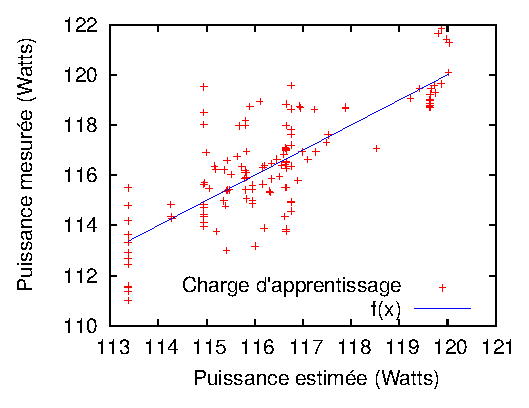
\includegraphics[width=0.45\textwidth]{chapitre5/chap5Fig/tpch-reg-poly-srv.eps}
  }
  \quad
  \subfloat[Modèle de régression en utilisant la configuration bas de gamme\label{fig:tpch-reg-poly-pc}]{
    \centering
    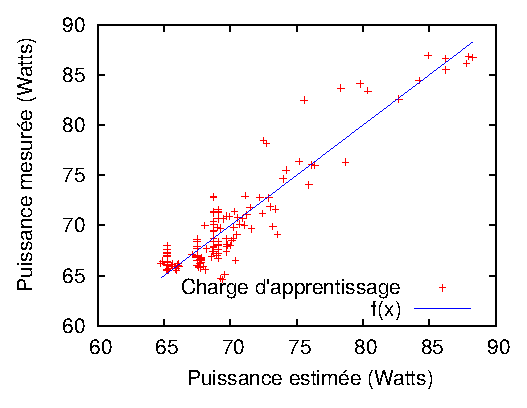
\includegraphics[width=0.45\textwidth]{chapitre5/chap5Fig/tpch-reg-poly-pc.eps}
  }
  \caption{La qualité du modèle de coût énergétique avec différent type de machine.}\label{fig:tpch-reg-postgres}
\end{figure}

Pour vérifier la portabilité de notre modèle de coût proposé contre les changements dans l'environnement matériel, nous menons cette expérimentation.
Les résultats de la phase d'apprentissage de notre modèle de coût pour les deux configurations sont représentés sur la \ref{fig:tpch-reg-postgres}. Comme nous pouvons le constater, la consommation d'énergie estimée et réelle, se rapprochent des lignes diagonales dans les deux configurations. Par ailleurs, dans la configuration du serveur, nous pouvons voir une variance entre la puissance estimée et observée pour certaines requêtes d'apprentissage. Une grande partie de ce résultat est due aux erreurs commises par l'optimiseur de requête du SGBD, dans l'estimation des coûts d'E/S et de CPU pour ces requêtes quand la taille du mémoire est grande. Ce phénomène classique a été rencontré pour une longue période par les optimiseurs de requêtes, et tous les modèles de performance proposés dans la littérature souffrent de ce problème, qui est lié à des erreurs d'estimation de cardinalités. En fait, les erreurs d'estimation dans les pipelines de bas niveau sont propagées aux niveaux supérieurs, et peuvent dégrader de manière significative la précision de la prédiction.

\subsubsection{Erreurs d'estimations du modèle de coût}\label{subsubsec:CostModelsErrorPostgres}
Dans ce type d'expérimentations, étant donné le coût de puissance estimé par notre modèle \textit{(E)}, on le compare avec la consommation de puissance active par le système \textit{(M)} réellement observée. Pour quantifier la précision du modèle, nous avons utilisé la métrique de taux d'erreur suivante : $Erreur = \frac{|M - E|}{M}$.
Pour tester notre modèle avec un grand ensemble de données, nous exécutons les 22 requêtes du benchmark TPC-H contre deux bases de données, avec un facteur d'échelle de 10 Go et de 100 Go. La plupart des requêtes contiennent plus de 4 pipelines. Les résultats sont présentés dans le \ref{tab:tpch-results-postgres-chap}.
Notez que certaines requêtes ont été arrêtés car ils ont dépassé les 72 heures d'exécution dans notre environnement de test en cours.

\begin{table}
\centering
\caption {Erreurs d'estimation d'énergie dans les requêtes du benchmark TPC-H avec différentes tailles de base de données.} \label{tab:tpch-results-postgres-chap}
\begin{tabular}{cccccc}
\toprule
%Requête & 10 Go & 100 Go & Requête & 10 Go & 100 Go \\
\multirow{2}{*}{\textbf{Requête}} & \multicolumn{2}{c}{\textbf{Erreur (\%)}} & \multirow{2}{*}{\textbf{Requête}} & \multicolumn{2}{c}{\textbf{Erreur (\%)}} \\ \cmidrule(lr){2-3} \cmidrule(l){5-6} 
    & \textbf{10 Go} & \textbf{100 Go} & & \textbf{10 Go} & \textbf{100 Go} \\
\midrule
	$Q1$& 1,03 & 0,2 & $Q11$ & 4,2 & - \\
	$Q2$& - & - & $Q12$ & 0,9 & 0,02 \\
	$Q3$& 1,5 & 1,2 & $Q13$ & 4,7 & 4,4 \\ 
	$Q4$& 0,6 & 0,5 & $Q14$ & 2,8 & 2,4 \\ 
	$Q5$& 1,2 & 3,07 & $Q15$ & 0,4 & 2,7 \\ 
	$Q6$& 4,1 & 2,7 & $Q16$ & 5,4 & 0,03 \\ 
	$Q7$& 0,4 & 1,4 & $Q18$ & 0,4 & - \\ 
	$Q8$& 0,07 & 1,09 & $Q19$ & 1,6 & 0,9 \\ 
	$Q10$& 0,6 & 0,3 & $Q22$ & 1,2 & 0,4 \\
\bottomrule
\end{tabular}
\end{table}

Comme nous pouvons le voir dans le tableau, l'erreur moyenne est généralement petite (0,1\% dans les deux ensembles de données 100 Go et 10 Go), et l'erreur maximale est habituellement inférieure à 5\%. L'expérimentation montre la précision de notre modèle de prédiction, indiquant qui est suffisamment précise pour l'employer dans un SGBD réel.

\subsubsection{Caractéristiques de requêtes}\label{subsubsec:QueryCharacterization}
Pour étudier les caractéristiques des 22 requêtes de TPC-H, nous procédons à une série de tests en utilisant \textit{EnerQuery}. Dans ces tests et pour chaque configuration (Temps-PG, Puissance-PG, Compromis-PG), nous exécutons tous les requêtes de TPC-H et nous collectons les estimations des coûts de performance et de puissance retournées par l'optimiseur de requêtes. Dans la \ref{fig:tpch-pg-conf} (les valeurs sont reportées sur une échelle logarithmique), nous pouvons constater que 16 des 22 requêtes ont le potentiel d'économie d'énergie dans la configuration Puissance-PG. Théoriquement, ce gain en économie d'énergie pour ces requêtes à un impact négatif sur le temps de traitement, comme indiqué dans la même figure. Cependant, le choix de la configuration compromis peut conduire à de bonnes valeurs d'économie d'énergie, avec moins de dégradation en terme de performances. Ces requêtes sont caractérisées par un nombre important d'opérateurs SQL et diverses opérations d'E/S et de CPU, ce qui donne à l'optimiseur de requêtes une variété de plans à choisir. Par conséquent, nous pouvons obtenir des requêtes avec une bonne économie d'énergie à partir de ces plans. D'autre part, le reste des requêtes qui ne peuvent pas bénéficier d'une économie d'énergie, sont des requêtes simples avec quelques tables et opérateurs SQL. Cela conduit l'optimiseur de requêtes à choisir le même plan dans toutes les configurations \textit{EnerQuery}, en raison du faible espace de recherche des plans.

\begin{figure}
  \centering
  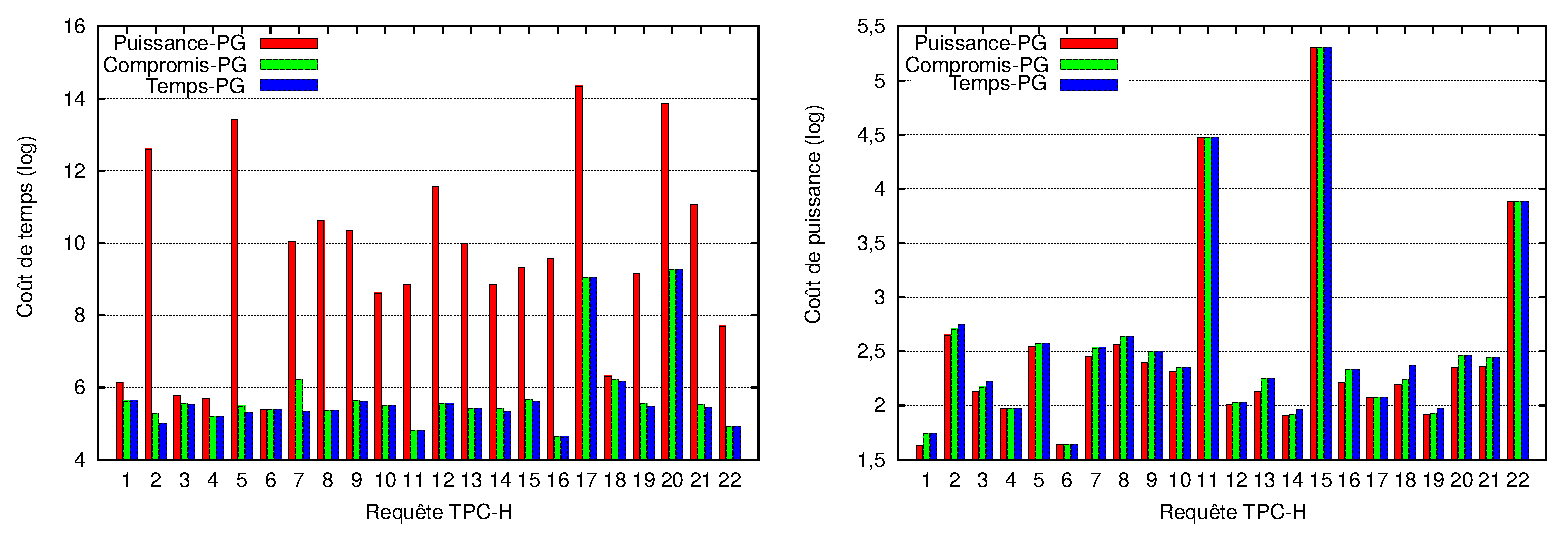
\includegraphics[width=1\textwidth]{chapitre5/chap5Fig/tpch-pg-conf.eps}
  \caption{Performance et puissance pour les requêtes de TPC-H en utilisant différentes configurations de \textit{EnerQuery}.}\label{fig:tpch-pg-conf}
\end{figure}

\subsubsection{Économie d'énergie et de puissance électrique}\label{subsubsec:PowerEnergySavingPostgres}
Le but de cette série d'expérimentations est d'étudier les avantages de notre approche en termes d'efficacité énergétique. Nous avons configuré le SGBD pour évaluer les coûts de performance et de consommation d'énergie pour les trois configurations (Temps-PG, Puissance-PG, Compromis-PG). Nous répétons les mêmes expérimentations avec deux tailles de bases de données différentes : 10 Go et 100 Go en utilisant le benchmark TPC-H.

\begin{figure}
  \centering
  \includegraphics[width=0.7\textwidth]{chapitre5/chap5Fig/power-time.pdf}
  \caption{Performance et économie d'énergie avec différentes configurations de \textit{EnerQuery} en utilisant TPC-H.}\label{fig:power-time}
\end{figure}

Dans la \ref{fig:power-time} nous présentons les résultats des expérimentations. On peut constater rapidement que la consommation est nettement plus faible quand on choisit une configuration d'optimiseur de requêtes favorisant les plans de faible puissance. Lorsque on compare les résultats d'une optimisation de puissance (Puissance-PG) avec une optimisation de performance (Temps-PG), on observe une grande marge en économie d'énergie, le bénéfice est remarquablement considérable dans la base de données de petite taille, peut-être cela est dû à la grande quantité des opérations d'E/S et le traitement des données requises par les requêtes exécutées dans cette base par rapport au bases de données de grande taille, qui se traduisent par plus de consommation d'énergie quel que soit le plan d'exécution choisi par l'optimiseur de requêtes.
Comme prévu, les économies de la configuration Compromis-PG sont plus petites que celles obtenues par la configuration favorisant la puissance, mais elles sont encore acceptables, en particulier dans des ensembles de données de 100 Go, elles sont approximatives.
D'autre part, la configuration de puissance prend plus de temps pour terminer l'exécution de toutes les requêtes, qui se traduit par une dégradation significative des performances. Ceci n'est pas surprenant, car si on gagne en puissance, on perd automatiquement en performances. Dans la configuration Compromis-PG, la dégradation des performances est en fait acceptable si on considère le gain de puissance atteint.

Notez que tous les résultats de nos expérimentations considèrent uniquement des économies d'énergie directes, dans un seul serveur de base de données. Ce nombre pourrait être encore plus élevé si on considère des centres de données à grande échelle avec des milliers de serveurs et de systèmes de refroidissement.

\section{Conclusion}
Dans ce chapitre, nous avons proposé un module de traitement de requête éco-énergétique \textit{EnerQuery} implémenté sur un SGBD réel qui est PostgreSQL. Avant de l'implémenter, une vérification a été effectuée pour identifier les composants du module de traitement de requêtes sensibles à l'énergie. En fonction de cette vérification, une méthodologie de construction d'un tel module a été donnée. Notre méthodologie est prise en charge par un outil open source disponible à la forge de notre laboratoire, pour permettre aux chercheurs, industriels et étudiants d'en tirer des profits. Des expérimentations intensives ont été menées pour démontrer l'efficacité et l'utilité de notre proposition. Les résultats obtenus sont très encourageants puisqu'ils démontrent des gains important en termes d’économie d’énergie et leurs influences sur les plans d’exécution étudiés.
